\newpage
\section{36. 有效的数独}
\label{leetcode:36}

\subsection{题目}

判断一个 9x9 的数独是否有效。只需要\textbf{根据以下规则},验证已经填入的数字是否有效即可。

\begin{enumerate}
  \item 数字 1-9 在每一行只能出现一次。
  \item 数字 1-9 在每一列只能出现一次。
  \item 数字 1-9 在每一个以粗实线分隔的 3x3 宫内只能出现一次。
\end{enumerate}

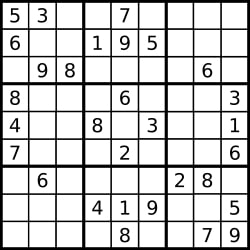
\includegraphics[width=60mm,height=60mm]{images/leetcode/36_sudo.jpg}

上图是一个部分填充的有效的数独。

数独部分空格内已填入了数字,空白格用 \verb|'.'| 表示。

\textbf{示例 1}:

\begin{verbatim}
输入:
[
  ["5","3",".",".","7",".",".",".","."],
  ["6",".",".","1","9","5",".",".","."],
  [".","9","8",".",".",".",".","6","."],
  ["8",".",".",".","6",".",".",".","3"],
  ["4",".",".","8",".","3",".",".","1"],
  ["7",".",".",".","2",".",".",".","6"],
  [".","6",".",".",".",".","2","8","."],
  [".",".",".","4","1","9",".",".","5"],
  [".",".",".",".","8",".",".","7","9"]
]
输出: true
\end{verbatim}

\textbf{示例 2}:

\begin{verbatim}
输入:
[
  ["8","3",".",".","7",".",".",".","."],
  ["6",".",".","1","9","5",".",".","."],
  [".","9","8",".",".",".",".","6","."],
  ["8",".",".",".","6",".",".",".","3"],
  ["4",".",".","8",".","3",".",".","1"],
  ["7",".",".",".","2",".",".",".","6"],
  [".","6",".",".",".",".","2","8","."],
  [".",".",".","4","1","9",".",".","5"],
  [".",".",".",".","8",".",".","7","9"]
]
输出: false
解释: 除了第一行的第一个数字从 5 改为 8 以外,空格内其他数字均与 示例1 相同。
     但由于位于左上角的 3x3 宫内有两个 8 存在, 因此这个数独是无效的。
\end{verbatim}

\textbf{说明}:

\begin{itemize}
  \item 一个有效的数独(部分已被填充)不一定是可解的。
  \item 只需要根据以上规则,验证已经填入的数字是否有效即可。
  \item 给定数独序列只包含数字 1-9 和字符 '.' 。
  \item 给定数独永远是 9x9 形式的。
\end{itemize}

\subsection{参考题解}

\subsubsection{Python}

\begin{verbatim}
class Solution:
  def isValidSudoku(self, board: List[List[str]]) -> bool:
    rows = len(board)
    cols = len(board[0])
    for row in range(rows):
      for col in range(cols):
        if board[row][col] == ".":
          continue
        c = board[row][col]
        board[row][col] = "."
        if not self.isValid(board, row, col, c):
          return False
        board[row][col] = c
    return True

  def isValid(self, board, row, col, c):
    for i in range(9):
      if board[i][col] == c:
        return False
      if board[row][i] == c:
        return False
      if board[row // 3 * 3 + i // 3][col // 3 * 3 + i % 3] == c:
        return False
    return True
\end{verbatim}
